\chapter{Programmazione greedy}
Gli algoritmi realizzati per risolvere \emph{problemi di ottimizzazione}
eseguono una sequenza di decisioni che nel caso della \emph{programmazione
dinamica} sono prese in maniera bottom-up e vengono valutate tutte le possibilità,
evitando però di ripetere decisioni già esaminate. Con la \emph{programmazione
greedy} invece, tra tutte le possibili decisioni ne viene scelta solo una,
quella che sembra ottima, o meglio localmente ottima. Tuttavia, è necessario
dimostrare che quella particolare scelta permetta di ottenere un risultato
ottimo anche a livello globale.

Proprio per questo motivo, la \emph{programmazione greedy} è utilizzabile sono
per quei problemi che presentano una \emph{sottostruttura ottima} e per i
quali è possibile dimostrare che esiste una scelta \q{ingorda}, cioè una scelta
che porta ad una soluzione ottima.

\section{Problema del resto}
\begin{problem}[Problema del resto]
    Dati un insieme di \q{tagli} di monete, espressi come vettore $t[1\dots n]$
    di interi positivi, e un valore $R$ rappresentate un resto da dover restituire,
    trovare il più piccolo numero intero di pezzi necessari per dare un resto
    $R$ di centesimi utilizzando i tagli disponibili, assumendo di avere un
    numero illimitato di monete.

    Formalmente, è necessario trovare un vettore di $x$ di interi non negativi
    tale che:
    \[R=\sum_{i=1}^n x[i]\cdot t[i]\quad\text{e}\quad m=\sum_{i=1}^n x[i]\quad
    \text{ha valore minimo}\]
\end{problem}

\noindent
Questo problema possiede una \emph{sottostruttura ottima}:
\begin{definition}[Sottostruttura ottima]
    Siano $S(i)$ il problema di dare un resto pari ad $i$ e $A(i)$ una soluzione
    ottima del problema $S(i)$, rappresentata da un multi-insieme. Sia poi
    $j\in A(i)$. Allora, $S(i-t[j])$ è un sotto-problema di $S(i)$, la cui
    soluzione è data da $A(i)-\{j\}$.
\end{definition}

\subsection{Approccio basato su programmazione dinamica}
Prima di vedere come potrebbe essere realizzata una soluzione \emph{greedy},
utilizziamo le proprietà della \emph{sottostruttura ottima} per implementare
una soluzione basata su \emph{programmazione dinamica}.

\noindent
Se $DP[i]$ rappresenta il numero minimo di monete necessario a risolvere il
problema $S(i)$, vale la seguente funzione ricorsiva:
\[DP[i]=\begin{cases}
    0 & i=0\\
    \min_{1\leq j\leq n}\{DP[i-t[j]]\;|\;t[j]\leq i\}+1 & i>0
\end{cases}\]

\begin{minicode}{Soluzione basata su programmazione dinamica}
\ind\bc{int}[] moneyChange(\bc{int}[] t, \bc{int} n, \bc{int} R)\\
    \bc{int}[] DP = new \bc{int}[0\dots R]\hfill\com{\emph{Tabella delle soluzioni}}
    \bc{int}[] coin = new \bc{int}[0\dots R]\hfill\com{Moneta da usare per uno specifico resto}
    DP[0] = 0\\
    \indf for (i = 1 to R) do\\
        DP[i] = $+\infty$\\
        \indff for (j = 1 to n) do\\
            \indfff if (i > t[j] and DP[i - t[j]] + 1 < DP[i]) then
                DP[i] = DP[i - t[j]] + 1\\
                coin[i] = j\\
    \indf\com{Ricostruzione della soluzione}
    \indf\bc{int}[] x = new \bc{int}[1\dots n] = \{0\}\hfill\com{Contatore delle monete usate}
    \indf while (R > 0) do\\
        x[coin[R]] = x[coin[R]] + 1\\
        R = R - t[coin[R]]\\
    \indf return x
\end{minicode}

\paragraph{Complessità}
La \emph{complessità} di questa soluzione è $\Theta(nR)$ per la presenza dei
due cicli annidati.

\subsection{Approccio basato su programmazione greedy}
Non è difficile immaginare che per minimizzare il numero di monete utilizzate
sia sufficiente usare sempre il taglio più grande possibile. Ovvero, selezionare
la moneta $j$ più grande, tale per cui $t[j]<R$, e risolvere il sotto-problema
$S(R-t[j])$.

\begin{minicode}{Soluzione basata su programmazione greedy}
\ind\bc{int}[] moneyChange(\bc{int}[] t, \bc{int} n, \bc{int} R)\\
    \bc{int}[] x = new \bc{int}[1\dots n]\\
    \{ \text{Ordina le monete in modo decrescente} \}\\
    \indf for (i = 1 to n) do\\
        x[i] = $\lfloor$R / t[i]$\rfloor$\\
        R = R - x[i] $\cdot$ t[i]\\
    \indf return x
\end{minicode}

\paragraph{Complessità}
Questa soluzione abbassa la \emph{complessità} a $O(n\log n)$ se l'insieme di
monete non è ordinato, $O(n)$ altrimenti.

\bigskip\noindent
Ciò che dobbiamo fare adesso è dimostrare che la scelta fatta sia corretta.

\begin{proof}[Dimostrazione]
    Supponiamo $t=[50, 10, 5, 1]$. Sia $x$ una qualunque soluzione ottima, ovvero
    tale per cui:
    \[R=\sum_{i=1}^n x[i]\cdot t[i]\quad\text{e}\quad m=\sum_{i=1}^n x[i]\quad
    \text{ha valore minimo}\]
    Sappiamo che $t[k]\cdot x[k]<t[k-1]$ altrimenti basterebbe sostituire un certo
    numero di monete di taglia $t[k]$ con quelle del taglio $t[k-1]$. In questo
    caso, i limiti al numero di monete per ogni taglio sono:
    \[\begin{array}{rclccclcl}
        t[2]\cdot x[2] & = & 10\cdot x[2] & < & t[1] & = & 50 & \Rightarrow & x[2]<5\\
        t[3]\cdot x[3] & = & 5\cdot x[3] & < & t[2] & = & 10 & \Rightarrow & x[3]<2\\
        t[4]\cdot x[4] & = & 1\cdot x[4] & < & t[3] & = & 5 & \Rightarrow & x[4]<5\\
    \end{array}\]
    Sia ora $m_k$ la somma delle monete di taglio inferiore a $t[k]$:
    \[m_k=\sum_{i=k+1}^4 x[i]\cdot t[i]\]
    Se riusciamo a dimostrare che $\forall k\;:\;m_k<t[k]$, allora la soluzione
    proposta dall'algoritmo è proprio quella ottima. Per ogni valore di $k$
    otteniamo:
    \[\begin{array}{rclclclclc}
        m_4 & = & 0 & & & < & 1 & & & =t[4]\\
        m_3 & = & x[4]\cdot1+m_4 & \leq & 4\cdot 1+m_4 & < & 4+1 & = & 5 & =t[3]\\
        m_2 & = & x[3]\cdot1+m_3 & \leq & 1\cdot 5+m_3 & < & 5+5 & = & 10 & =t[2]\\
        m_1 & = & x[2]\cdot1+m_2 & \leq & 4\cdot 10+m_2 & < & 40+10 & = & 50 & =t[1]\\
    \end{array}\]
\end{proof}
\begin{note}
    Non tutti i tagli di monete permettono di utilizzare la \emph{programmazione
    greedy}. Ad esempio, per $t[10,8,1]$ l'algoritmo \emph{greedy} utilizzerebbe
    una moneta da 10 e 7 da 1, quando la scelta migliore sarebbe quella di
    prenderne 2 da 8 e una da 1.
\end{note}
\begin{note}
    In ogni caso, l'insieme delle monete deve includere una moneta di taglio
    unitario.
\end{note}

\section{Insieme indipendente massimale di intervalli}
Vediamo un caso particolare del problema sulla \nameref{prob:12} in cui il peso
di tutti gli intervalli è $1$. Cioè vogliamo cercare l'insieme contenente il
maggior numero di intervalli.

\begin{figure}[h!]
    \centering
    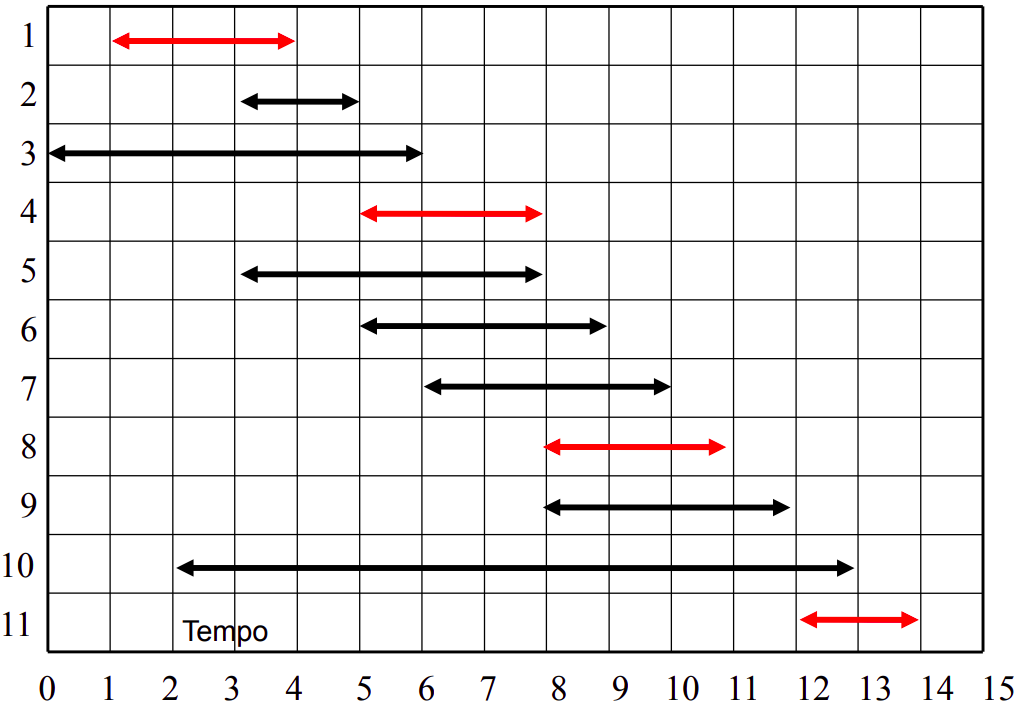
\includegraphics[width=0.45\textwidth]{intervalli-ordinati-greedy1.png}
    \caption{Possibile soluzione}
\end{figure}

\subsection{Approccio basato su programmazione dinamica}
Iniziamo ricercando una \emph{sottostruttura ottima}. Assumiamo che gli intervalli
siano ordinati per tempo di fine:
\[b_1\leq\dots\leq b_n\]
Definiamo il sotto-problema $S[i\dots j]$ come l'insieme di intervalli che
iniziano dopo la fine di $i$ e finiscono prima dell'inizio di $j$:
\[S[i\dots j]=\{k\;|\;b_i\leq a_k<b_k\leq a_j\}\]
Aggiungiamo due intervalli fittizi:
\begin{itemize}
    \item \emph{Intervallo $0$}: $b_0=-\infty$;
    \item \emph{Intervallo $n+1$}: $a_{n+1}=+\infty$;
\end{itemize}
Il problema generale corrisponde quindi al problema $S[0\dots n+1]$.

\begin{definition}[Sottostruttura ottima]
    Supponiamo che $A[i\dots j]$ sia una soluzione ottimale di $S[i\dots j]$
    e sia $k$ un intervallo che appartiene ad $A[i\dots j]$. Allora:
    \begin{itemize}
        \item Il problema $S[i\dots j]$ può essere suddiviso in due intervalli:
        \begin{enumerate}
            \item $S[i\dots k]$ contiene gli intervalli di $S[i\dots j]$ che
            finiscono prima di $k$;
            \item $S[k\dots j]$ contiene gli intervalli di $S[i\dots j]$ che
            iniziano dopo $k$;
        \end{enumerate}
        \item $A[i\dots j]$ contiene le soluzioni ottimali di $S[i\dots k]$ e
        $S[k\dots j]$:
        \begin{enumerate}
            \item $A[i\dots j]\cap S[i\dots k]$ è la soluzione ottimale di $A[i\dots k]$;
            \item $A[i\dots j]\cap S[k\dots j]$ è la soluzione ottimale di $A[k\dots j]$;
        \end{enumerate}
    \end{itemize}
\end{definition}

\noindent
Quanto detto ci permette di definire $A[i\dots j]$ come:
\[A[i\dots j]=A[i\dots k]\cup\{k\}\cup A[k\dots j]\]
Per determinare $k$ proviamo tutte le possibilità. A questo punto, sia $DP[i][j]$
la dimensione del più grande sottoinsieme $A[i\dots j]\subseteq S[i\dots j]$ di
intervalli indipendenti. Possiamo definire $DP[i][j]$ con la seguente funzione
ricorsiva:
\[DP[i][j]=\begin{cases}
    0 & S[i\dots j]=\emptyset\\
    \max_{k\in S[i\dots j]}\{DP[i][k]+DP[k][j]+1\} & \text{altrimenti}
\end{cases}\]
Questa definizione ci permette di realizzare un algoritmo basato su
\emph{programmazione dinamica} o \emph{memoization} con \emph{complessità} $O(n^3)$
perché bisogna risolvere tutti i problemi con $i<j$ e, nel caso peggiore,
paghiamo $O(n)$ per ogni sotto-problema.

\bigskip\noindent
Possiamo fare meglio di così?

Potremmo semplicemente usare la soluzione al problema con pesi generici, che
ha \emph{complessità} $O(n\log n)$, ponendo a $1$ tutti i pesi. Tuttavia,
possiamo chiederci se sia davvero necessario analizzare tutti i possibili valori
di $k$. Definiamo il seguente teorema:

\begin{definition}[Scelta ingorda]
    Siano $S[i\dots j]$ un sotto-problema non vuoto e $m$ l'intervallo di $S[i\dots
    j]$ con il minor tempo di fine. Allora, valgono i due seguenti punti:
    \begin{enumerate}
        \item Il sotto-problema $S[i\dots m]$ è vuoto;
        \item $m$ è compreso in una qualche soluzione ottima di $S[i\dots j]$,
        ovvero $m\in A[i\dots j]$;
    \end{enumerate}
\end{definition}
\begin{proof}[Dimostrazione]
    Dimostriamo separatamente i due punti.

    \paragraph{Punto 1 - \bm{$S[i$}\dots\bm{$ j]=\emptyset$}}
    Per la definizione di intervallo sappiamo che $a_m<b_m$. Inoltre, poiché $m$
    è l'intervallo con il minor tempo di fine $\forall k\in S[i\dots j]$ $b_m
    \leq b_k$ e, quindi, ne consegue che $\forall k\in S[i\dots j]$ $a_m<b_k$.

    Se nessun intervallo in $S[i\dots j]$ termina prima di $a_m$, allora $S[i
    \dots m]=\emptyset$.

    \paragraph*{Punto 2 - \bm{$m\in A[i$}\dots\bm{$i]$}}
    Siano $A'[i\dots j]$ una soluzione ottima di $S[i\dots j]$ e $m'$ l'intervallo
    con minor tempo di fine in $A'[i\dots j]$. Sia ora $A[i\dots j]=A'[i\dots j]
    -\{m'\}\cup\{m\}$ una nuova soluzione ottima ottenuta togliendo $m'$ e
    aggiungendo $m$ ad $A'[i\dots j]$. $A[i\dots j]$ è una soluzione ottima che
    contiene $m$ in quanto ha la stessa cardinalità di $A'[i\dots j]$ e gli
    intervalli sono indipendenti.
\end{proof}

\noindent
Questa dimostrazione ci permette di selezionare sempre gli intervalli con tempo
di fine minore e ignorare tutti quelli che si intersecano con esso, riducendo
il problema alla ricerca dell'\emph{insieme indipendente massimale} in $S[m\dots
j]$.

\begin{figure}[h!]
    \centering
    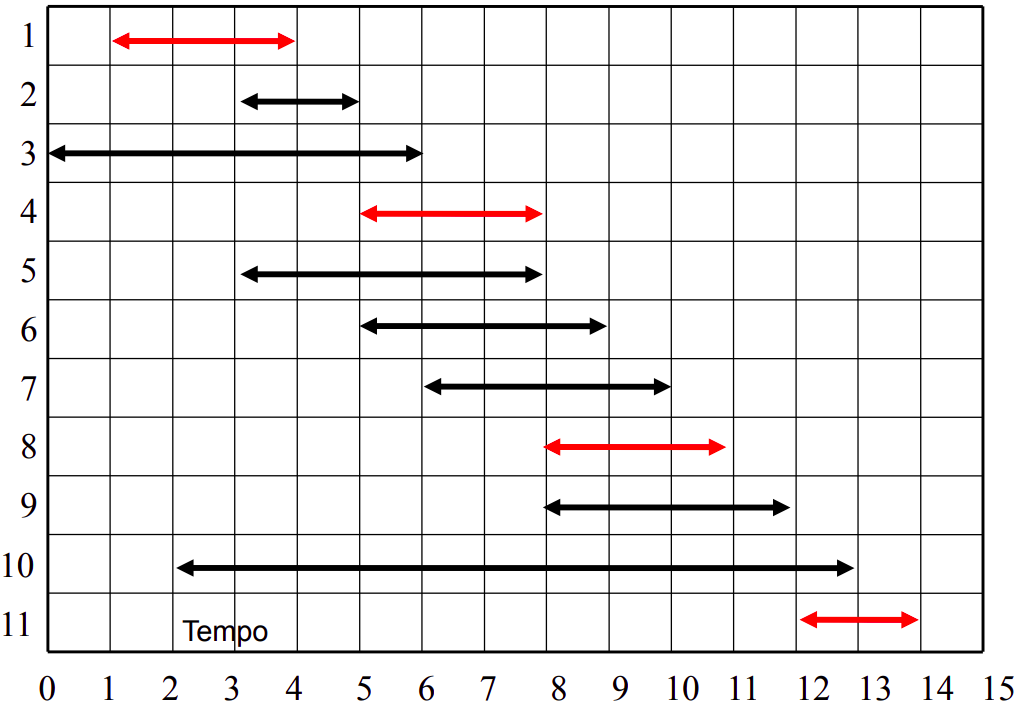
\includegraphics[width=0.45\textwidth]{intervalli-ordinati-greedy1.png}
    \caption{Soluzione con \emph{scelte ingorde}}
\end{figure}

\begin{minicode}{Soluzione basata su programmazione greedy}
\ind\bc{SET} indipendentSet(\bc{int}[] a, \bc{int}[] b)\\
    \{ Ordina i vettori $a$ e $b$ in modo che $b_1\leq\dots\leq b_n$ \}\\
    \bc{SET} S = Set()\\
    S.insert(1)\\
    \bc{int} last = 1\\
    \indf for (i = 2 to n) do\\
        \indff if (a[i] $\geq$ b[last]) then\\
            S.insert(i)\\
            last = i\\
    \indf return S
\end{minicode}

\paragraph{Complessità}
Questa soluzione abbassa la \emph{complessità} a $O(n)$ se i vettori di input
sono già ordinati, $O(n\log n)$ altrimenti.

\begin{eg}[Esempio d'esecuzione]
    Eseguendo l'algoritmo con gli stessi insiemi degli esempi precedenti
    l'algoritmo fa le seguenti scelte:

    \begin{figure}[h!]
        \centering
        \subfloat{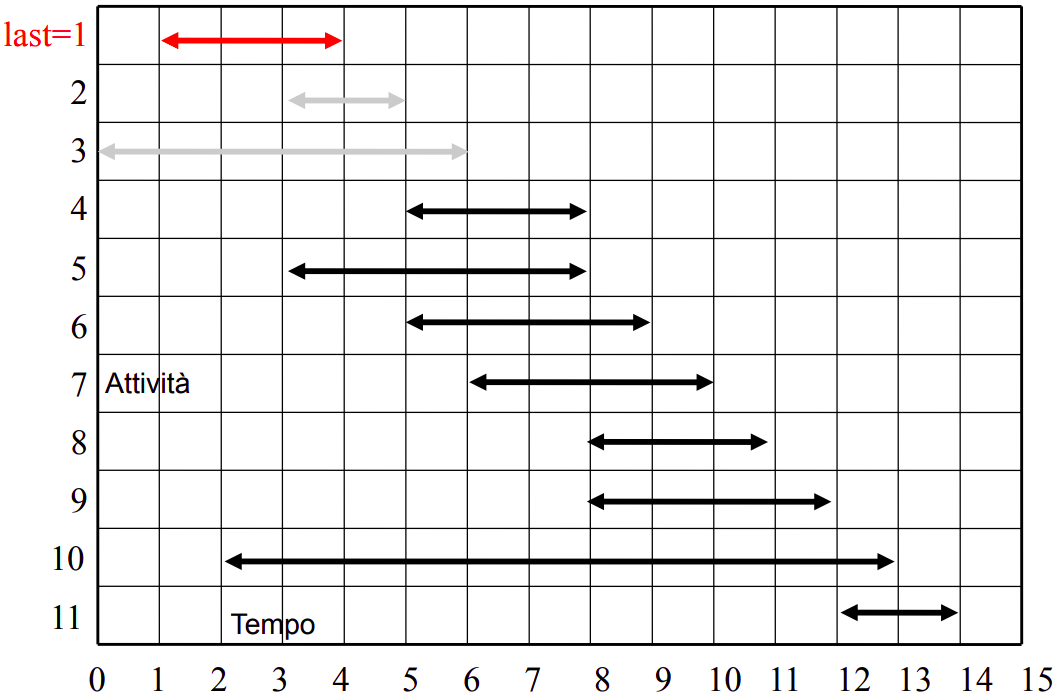
\includegraphics[width=0.48\textwidth]
        {intervalli-ordinati-greedy-s1.png}}
        \hfill
        \subfloat{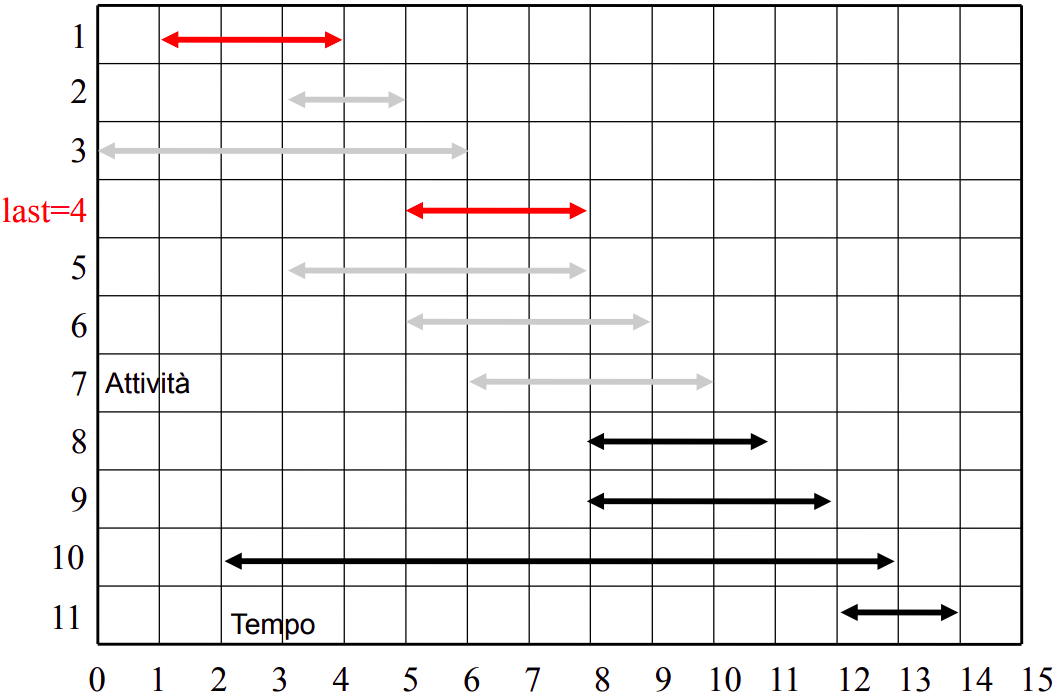
\includegraphics[width=0.48\textwidth]
        {intervalli-ordinati-greedy-s2.png}}\\
        \subfloat{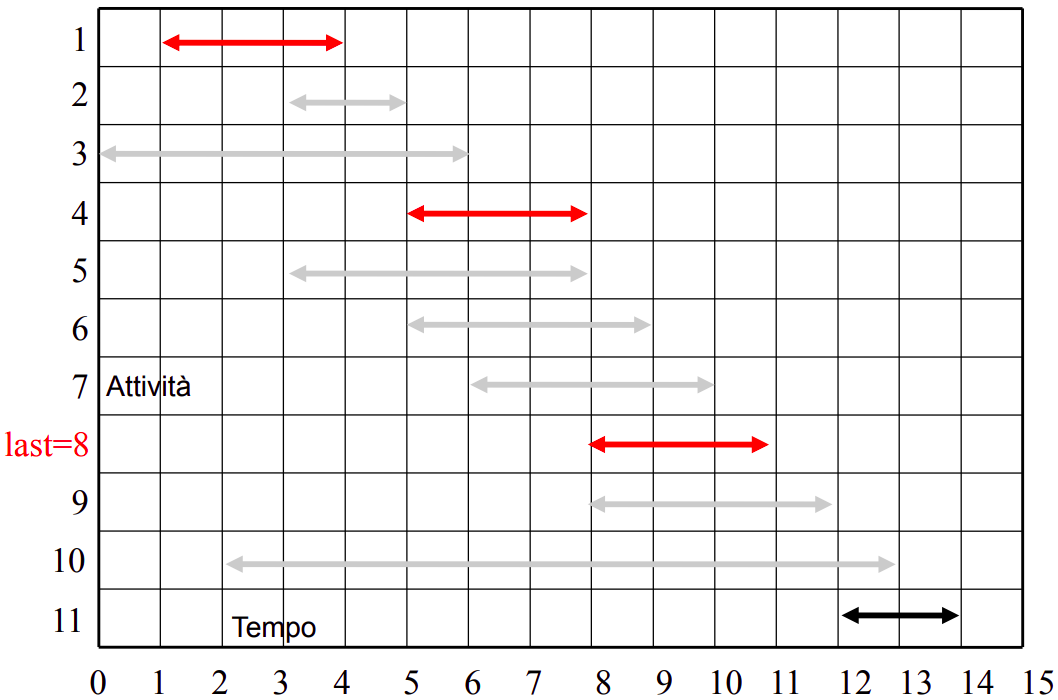
\includegraphics[width=0.48\textwidth]
        {intervalli-ordinati-greedy-s3.png}}
        \hfill
        \subfloat{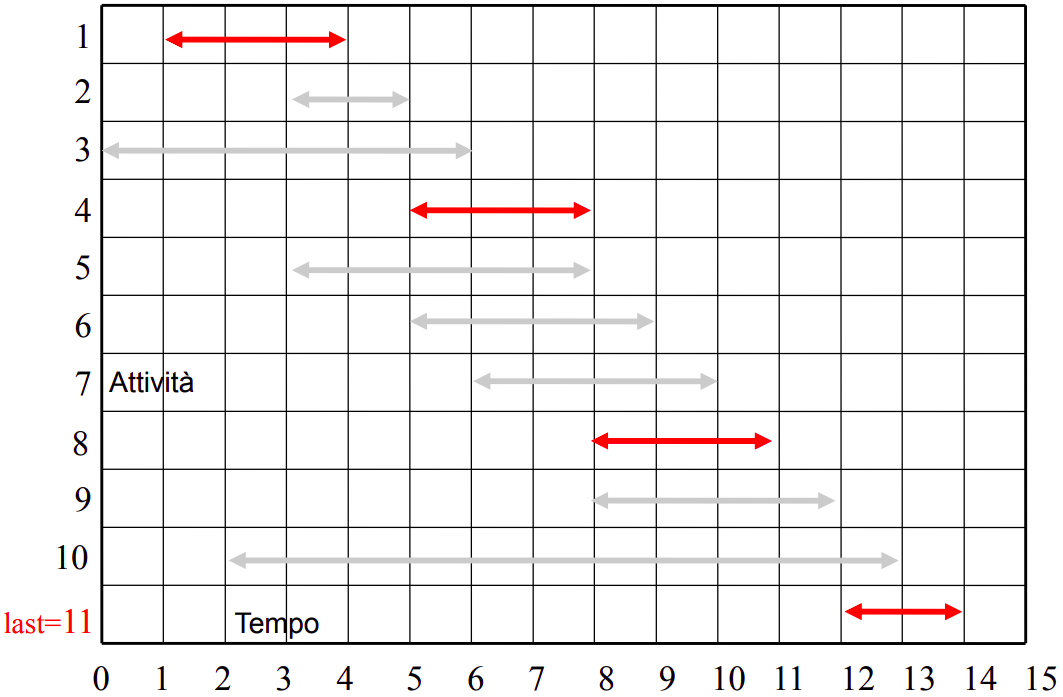
\includegraphics[width=0.48\textwidth]
        {intervalli-ordinati-greedy-s4.png}}
    \end{figure}
\end{eg}

\section{Problema dello scheduling}
\begin{problem}[Scheduling dei processi]
    Dati un processore e $n$ processi da eseguire su di esso. Se ogni processo $i$
    è caratterizzato da un tempo d'esecuzione $t[i]$ noto a priori, trovare una
    sequenza d'esecuzione che minimizzi il tempo di completamento medio.
\end{problem}
\begin{definition}[Tempo di completamento]
    Dato un vettore $A[1\dots n]$ contenente una permutazione di $\{1\dots n\}$,
    il tempo di completamento dell'$h$-esimo processo nella permutazione è
    calcolato come:
    \[T_A(h)=\sum_{i=1}^h t[A[i]]\]
\end{definition}

\newpage
\begin{eg}[Possibili permutazioni]
    Consideriamo i seguenti processi con relativo tempo d'esecuzione:
    
    \begin{table}[h!]
        \centering
        \renewcommand{\arraystretch}{1.2}
        \begin{tabular}{|c|c|c|c|c|}
            \hline
            \textbf{Processo} & $1$ & $2$ & $3$ & $4$\\
            \hline
            \bm{$t[i]$} & 4 & 1 & 6 & 3\\
            \hline
        \end{tabular}    
    \end{table}

    \noindent
    Se eseguissimo i processi nell'ordine $A[1,2,3,4]$ la situazione sarebbe
    la seguente:

    \begin{figure}[h!]
        \centering
        \begin{graph}
            \tikzset{
                cell/.style={rectangle, draw, minimum size=10mm, anchor=west},
            }
            \node[cell] (1) [minimum width=40mm, label={[xshift=-12mm]225:{$0$}}] {$4$};
            \node[cell] (2) [minimum width=10mm, right of=1, xshift=5mm,
            label={[xshift=3mm]225:{$4$}}, label={[xshift=-3mm]-45:{$5$}}] {$1$};
            \node[cell] (3) [minimum width=60mm, right of=2, xshift=15mm,
            label={[xshift=21.5mm]-45:{$11$}}] {$6$};
            \node[cell] (4) [minimum width=30mm, right of=3, xshift=25mm,
            label={[xshift=6mm]-45:{$14$}}] {$3$};
        \end{graph}
    \end{figure}

    \noindent
    Il tempo di completamento medio sarebbe:
    \[\frac{\sum_{i=1}^4 T_A(i)}{4}=\frac{4+5+11+14}{4}=\frac{34}{4}=8.5\]
    Se invece ordinassimo i processi per tempo d'esecuzione crescente, ponendo
    $A=[2,4,1,3]$, la situazione diventerebbe:
    
    \begin{figure}[h!]
        \centering
        \begin{graph}
            \tikzset{
                cell/.style={rectangle, draw, minimum size=10mm, anchor=west},
            }
            \node[cell] (2) [minimum width=10mm, label={[xshift=3mm]225:{$0$}},
            label={[xshift=-2.5mm]-45:{$1$}}] {$1$};
            \node[cell] (4) [minimum width=30mm, right of=2,
            label={[xshift=7mm]-45:{$5$}}] {$3$};
            \node[cell] (1) [minimum width=40mm, right of=4, xshift=15mm,
            label={[xshift=12mm]-45:{$8$}}] {$4$};
            \node[cell] (3) [minimum width=60mm, right of=1, xshift=30mm,
            label={[xshift=21.5mm]-45:{$14$}}] {$6$};
        \end{graph}
    \end{figure}

    \noindent
    Il tempo di completamento medio adesso è:
    \[\frac{\sum_{i=1}^4 T_A(i)}{4}=\frac{1+5+8+14}{4}=\frac{27}{4}=6.75\]
\end{eg}
\begin{note}
    Dall'esempio intuiamo che la scelta ottima potrebbe essere quella di
    prendere sempre il processo con minor \emph{tempo d'esecuzione}.
\end{note}

\begin{definition}[Scelta ingorda]
    Esiste una soluzione ottima $A$ in cui il processo con minor tempo
    d'esecuzione si trova in prima posizione.
\end{definition}

\begin{definition}[Sottostruttura ottima]
    Sia $A$ una soluzione ottima di un problema con $n$ processi, in cui il
    processo con minor tempo d'esecuzione $m$ si trova in prima posizione. La
    permutazione dei seguenti $n-1$ processi è una soluzione al sotto-problema
    in cui $m$ non viene considerato.
\end{definition}
\begin{proof}[Dimostrazione]
    Consideriamo una \emph{permutazione ottima} $A$:
    \[A=[A[1],\dots A[m],\dots,A[n]]\]
    Siano $m$ l'indice del processo con minor \emph{tempo d'esecuzione} e
    $A'$ una permutazione in cui i processi in posizione $1$ e $m$ vengono
    scambiati, ovvero:
    \[A=[A[m],\dots,A[1],\dots,A[n]]\]
    Il \emph{tempo di completamento medio} di $A'$ è minore o uguale a quello di
    $A$. Questo è vero perché i processi nelle posizioni $1,\dots,m-1$ in $A'$
    hanno un \emph{tempo di completamento} minore o uguale a quello dei processi
    in posizione $1,\dots,m-1$ in $A$. D'altra parte, i processi nelle posizioni
    $m,\dots,n$ hanno lo stesso \emph{tempo di completamento} sia in $A$ che in
    $A'$.

    Ora, poiché avevamo ipotizzato che $A$ fosse una \emph{permutazione ottima},
    il suo \emph{tempo di completamento medio} non può essere superiore a quello
    di $A'$, quindi anche $A'$ è una \emph{permutazione ottima}.
\end{proof}

\section{Problema dello zaino frazionario}
Consideriamo una variante del \emph{\hyperref[prob:7]{problema dello zaino}}
in cui è possibile prendere frazioni di oggetti.

\begin{eg}[Possibili ordinamenti degli oggetti]
    Consideriamo uno zaino con capacità 70 e di avere i tre oggetti seguenti:

    \begin{table}[h!]
        \centering
        \renewcommand{\arraystretch}{1.2}
        \begin{tabular}{|c|c|c|}
            \hline
            \bm{$i$} & \bm{$p_i$} & \bm{$w_i$}\\
            \hline
            1 & 60 & 10\\
            \hline
            2 & 200 & 40\\
            \hline
            3 & 120 & 30\\
            \hline
        \end{tabular}
    \end{table}

    \noindent
    Per prendere gli oggetti possiamo provare a ordinarli in qualche modo
    così poter operare una scelta ponderata sul tipo di ordinamento scelto.

    \paragraph{Ordinamento per profitto decrescente}
    In questo modo andremmo a scegliere gli oggetti $2$ e $3$ ottenendo un
    guadagno totale di $320$.

    \paragraph{Ordinamento per peso crescente}
    Questo approccio ci porterebbe a scegliere la totalità degli oggetti $1$
    e $3$, per un peso di $40$. Per usare la rimanente capacità prendiamo i
    $\frac{3}{4}$ dell'oggetto $2$. Il profitto che otteniamo sale quindi a
    $330$.

    \paragraph{Ordinamento per profitto specifico decrescente}
    Definiamo il profitto specifico come il rapporto $\frac{p_i}{w_i}$. Per gli
    oggetti $1$, $2$, $3$ il profitto specifico vale $6$, $5$ e $4$ rispettivamente.
    Di conseguenza, prendiamo la totalità degli oggetti $1$ e $2$ e i $\frac{2}{3}$
    dell'ultimo oggetto. Questa scelta ci assicura un guadagno di $340$.
\end{eg}
\begin{minicode}{Implementazione della soluzione}
\ind\bc{float}[] zaino(\bc{float}[] p, \bc{float}[] w, \bc{float} C, \bc{int} n)\\
    \bc{float}[] x = new \bc{float}[1\dots n]\hfill\com{Vettore delle quantità raccolte}
    \{ Ordina $p$ e $w$ in modo che $p[1]/w[1]\geq\dots\geq p[n]/w[n]$\}\\
    \indf for (i = 1 to n) do\\
        x[i] = min(C / w[i], 1)\\
        C = C - x[i] $\cdot$ w[i]\\
    \indf return x
\end{minicode}

\paragraph{Complessità}
La \emph{complessità} è $O(n)$ se i vettori di input sono già ordinati, $O(n\log
n)$ altrimenti.

\bigskip\noindent
Abbiamo definito l'algoritmo, ma in realtà non abbiamo ancora dimostrato che
quel tipo di scelta sia corretta.

\begin{proof}[Dimostrazione]
    Assumiamo che gli oggetti siano ordinati per \emph{profitto specifico
    decrescente}. Sia $x$ una soluzione ottima e supponiamo che $x[1]<\min\left(
    \frac{C}{w[i]}, 1\right)<1$. Allora, possiamo costruire una nuova soluzione
    in cui $x'[1]=\min\left(\frac{C}{w[i]}, 1\right)$ e la porzione di uno o
    più oggetti è ridotta di conseguenza. La soluzione $x'$ è sicuramente di
    profitto uguale o maggiore rispetto ad $x$ perché il \emph{profitto
    specifico} del primo oggetto è massimo.
\end{proof}

\section{Problema della compressione}
Quello della compressione dei dati è una problema classico dell'informatica.
Una delle possibili tecniche per la compressione dei caratteri\footnote{Per
le immagini esistono tecniche migliori} è tramite una \emph{funzione di codifica}
del tipo $f:f(c)=x$ in cui $c$ un carattere preso da un alfabeto $\Sigma$ e
$x$ è la sua rappresentazione binaria.

\begin{note}
    $\Sigma$ può essere definito come l'insieme dei caratteri usati all'interno
    di un file da comprimere.
\end{note}

\begin{eg}[Possibili compressioni]
    Supponiamo di avere un file di $n$ caratteri, che $\Sigma=\{a,b,c,d,e,f\}$ e
    di conoscere la frequenza di ogni carattere.

    \begin{table}[h!]
        \centering
        \renewcommand{\arraystretch}{1.2}
        \begin{adjustbox}{max width=0.98\textwidth}
        \begin{tabular}{|c|c|c|c|c|c|c|c|}
            \hline
            \textbf{Caratteri} & \bc{\texttt{a}} & \bc{\texttt{b}} &
            \bc{\texttt{c}} & \bc{\texttt{d}} & \bc{\texttt{e}} &
            \bc{\texttt{f}} & \textbf{Dimensione}\\
            \hline
            \textbf{Frequenza} & 45\% & 13\% & 12\% & 16\% & 9\% & 5\% & \\
            \hline
            \textbf{ASCII} & \texttt{01100001} & \texttt{01100010} &
            \texttt{01100011} & \texttt{01100100} & \texttt{01100101} &
            \texttt{01100110} & 8n\\
            \hline
            \textbf{Codifica 1} & \texttt{000} & \texttt{001} & \texttt{010} &
            \texttt{011} & \texttt{100} & \texttt{101} & 3n\\
            \hline
            \textbf{Codifica 2} & \texttt{0} & \texttt{101} & \texttt{100} &
            \texttt{111} & \texttt{1101} & \texttt{1100} & 2.24n\\
            \hline
        \end{tabular}
    \end{adjustbox}
    \end{table}
    
    \noindent
    Nella codifica 1 abbiamo codificato i caratteri usando il numero minimo
    minimo di bit necessari per rappresentare 6 valori. Per quanto riguarda la
    codifica 2 invece, abbiamo calcolato la dimensione totale come:
    \[\left(0.45\cdot1+0.13\cdot3+0.12\cdot3+0.16\cdot3+0.09\cdot4+0.05\cdot
    4\right)n=2.24n\]
\end{eg}

\begin{definition}[Codice a prefisso]
    In un codice a prefisso, nessun codice è prefisso di un altro.
\end{definition}\noindent
La caratteristica dei \emph{codici a prefisso} è necessaria per consentire la
decodifica.

\begin{eg}[Codici a prefisso e non]
    Consideriamo un codice del tipo:
    \[a\to0,\,b\to 10,\,c\to11\]
    La codifica per la stringa \texttt{babaca} è:
    \[10\ 0\ 10\ 0\ 11\ 0\]
    che può essere decodificata senza ambiguità percorrendola da sinistra, in
    quanto, appena viene riscontrata la corrispondenza con un carattere, si
    può sostituire quel carattere alla sua codifica sapendo che i bit successivi
    costituiranno la rappresentazione di un altro carattere.

    Nel caso di un codice di questo tipo invece:
    \[a\to0,\, b\to1,\,c\to 11\]
    dovendo decodificare la sequenza di bit:
    \[111111\]
    si crea un'ambiguità in quanto un singolo bit $1$ rappresenta la $b$, mentre
    due bit rappresentano la $c$.
\end{eg}

\subsection{Algoritmo di Huffman}
L'\emph{algoritmo di Huffman} utilizza rappresentazioni ad albero per definire
il codice di codifica a partire dal testo e per ritornare al testo originale a
partire dalla codifica.